Sean a,b>0. Resolver \(u_{xx}+u_{yy}=0\) en \(0<x<a,0<y<b\), con
\[u(x,0)=u(0,y)=u(a,y)=0,\qquad u(x,b)=g(x).\]
Para interpretar las condiciones en toda la frontera, suponer g continua, suave por tramos,
con g(0)=g(a)=0 y derivadas por tramos suficientes para la expansión seno.

\begin{enumerate}[label=(\alph*),ref=\alph*,leftmargin=*]
\item Determinar la solución para una función g dada.
\item Resolver para \(g(x)=x\) si0\ensuremath{\le}x\ensuremath{\le}a/2 y \(g(x)=a-x\) si a/2\ensuremath{\le}x\ensuremath{\le}a.
\end{enumerate}

\Needspace{7.46cm}
\begin{center}
\begin{minipage}{\linewidth}
\centering
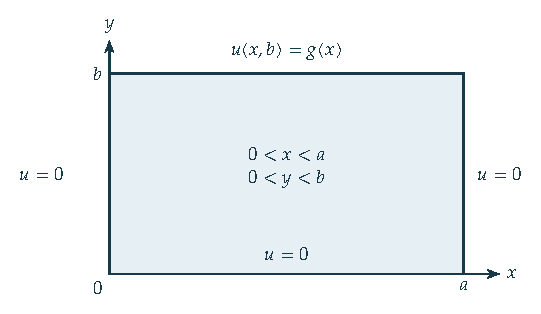
\includegraphics[width=10.25cm]{assets/M2-E0109-setup.pdf}\par
\smallskip{\small Dominio rectangular y datos prescritos en sus cuatro lados.\par}
\end{minipage}
\end{center}
